% Requires: \usepackage{subcaption} \usepackage{graphicx}
% Image paths are relative to this .tex file's location.
% Generated by: smixae latex figures  (experiment: gemma_2_9b_l20)

\begin{figure*}[t]
\centering
\begin{minipage}[t]{0.49\linewidth}
  \centering
  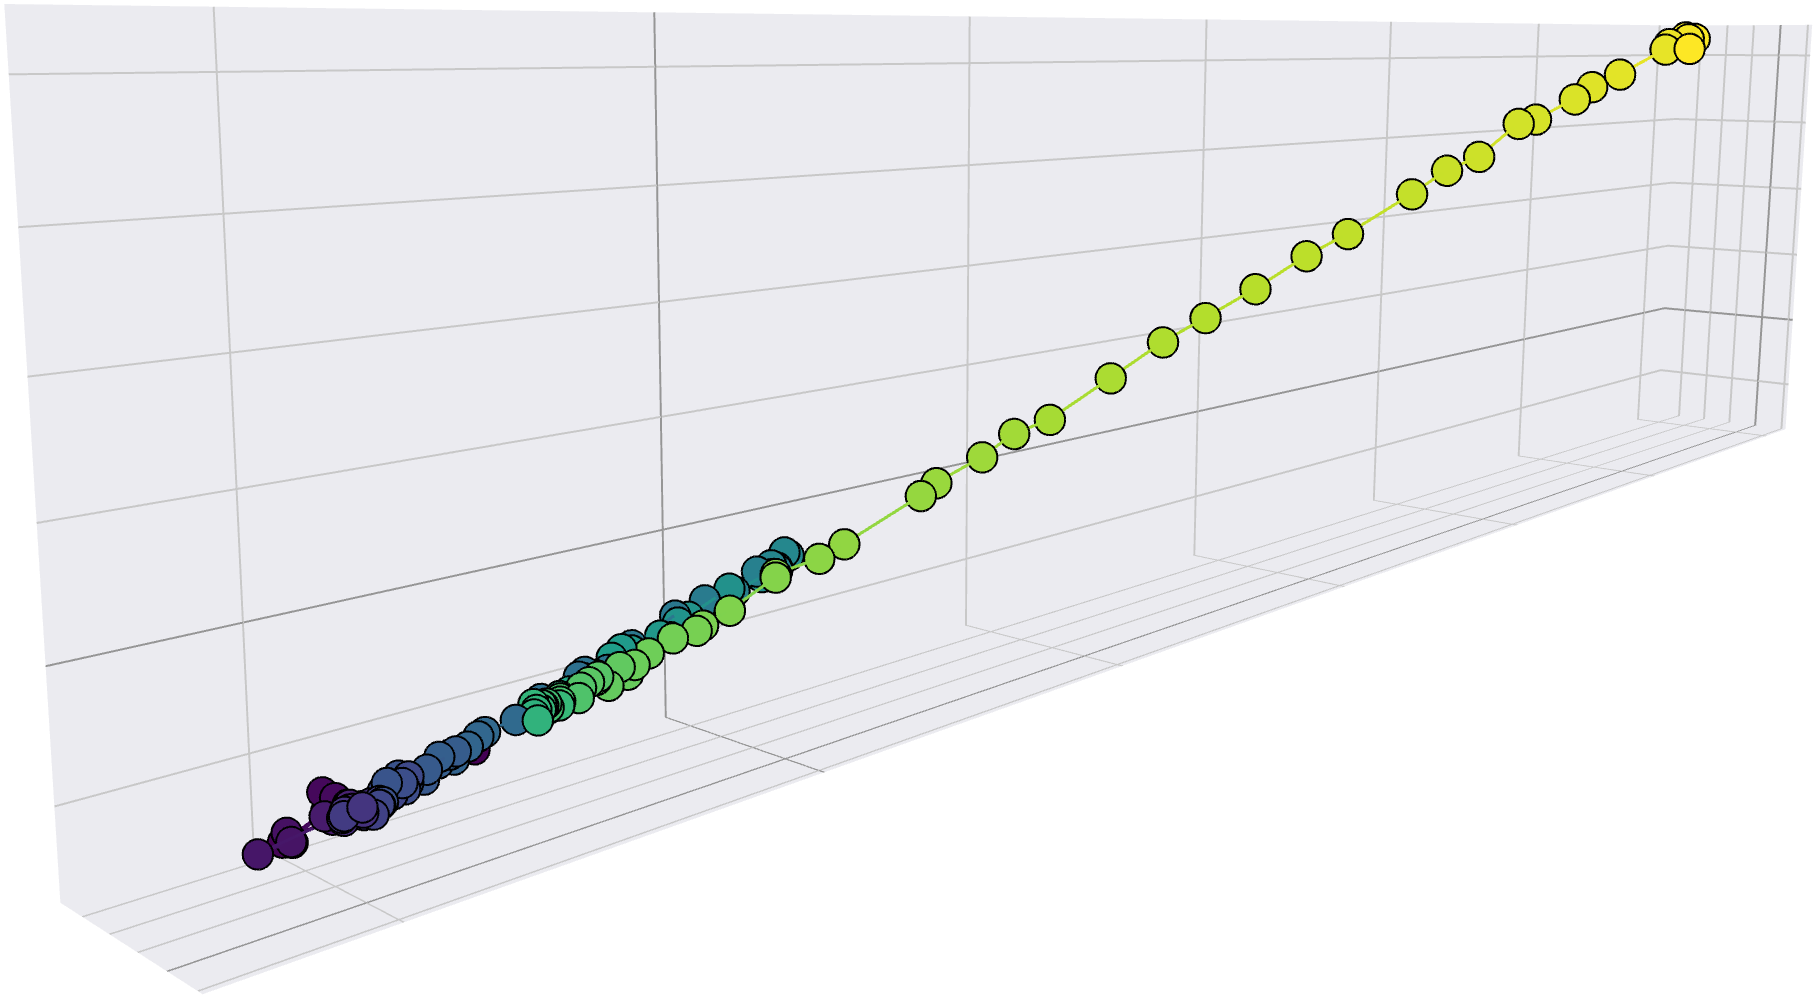
\includegraphics[width=0.85\linewidth]{camera_ready/gemma_2_9b_l20__pile-uncopyrighted__E1749__periodic_gain__per_gain__0.3201__means.png}
  \\[2pt]
  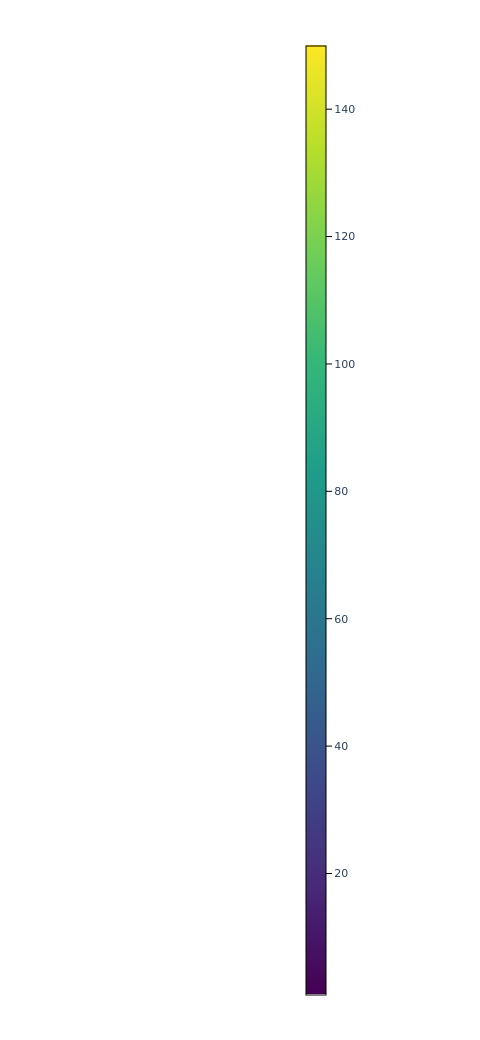
\includegraphics[width=0.7\linewidth]{legends/legend_pile-uncopyrighted__150.png}
\end{minipage}\hfill
\begin{minipage}[t]{0.49\linewidth}
  \centering
  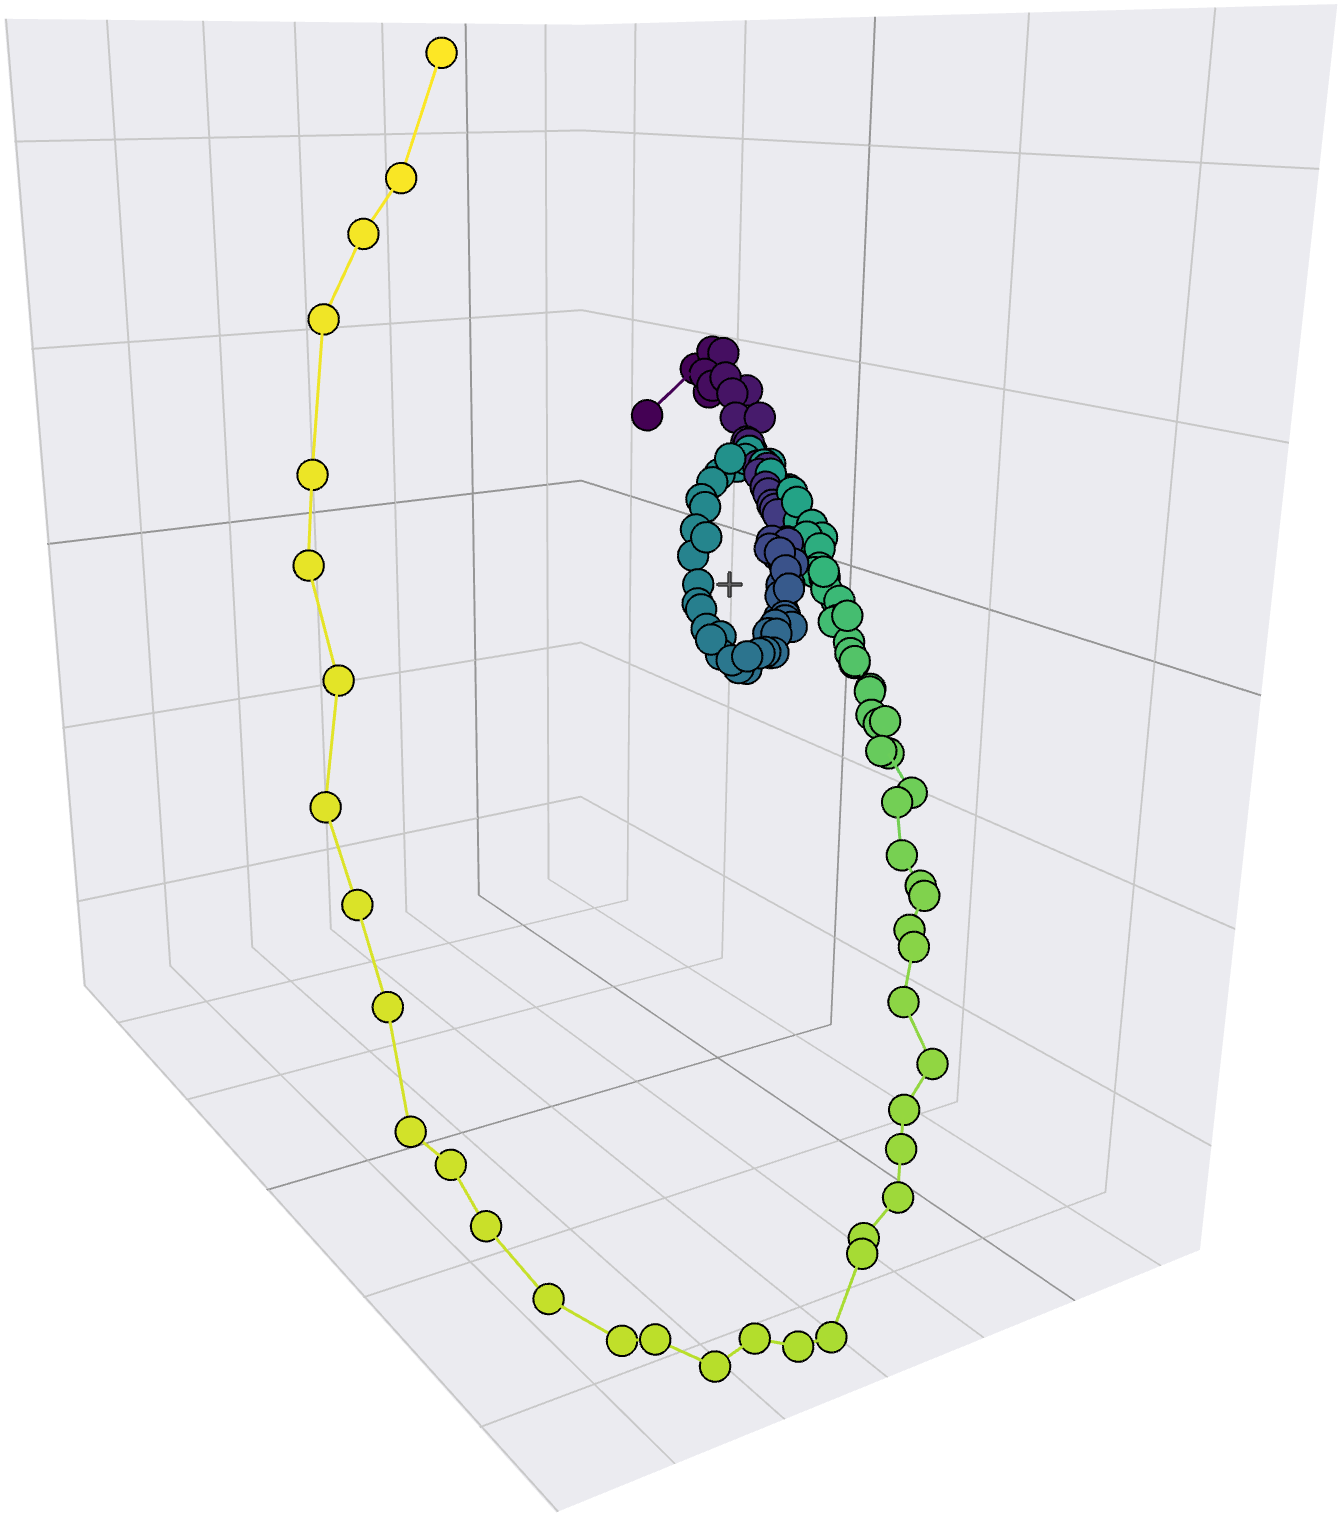
\includegraphics[width=0.85\linewidth]{camera_ready/gemma_2_9b_l20__pile-uncopyrighted__E1520__periodic_gain__per_gain__0.2844__means.png}
  \\[2pt]
  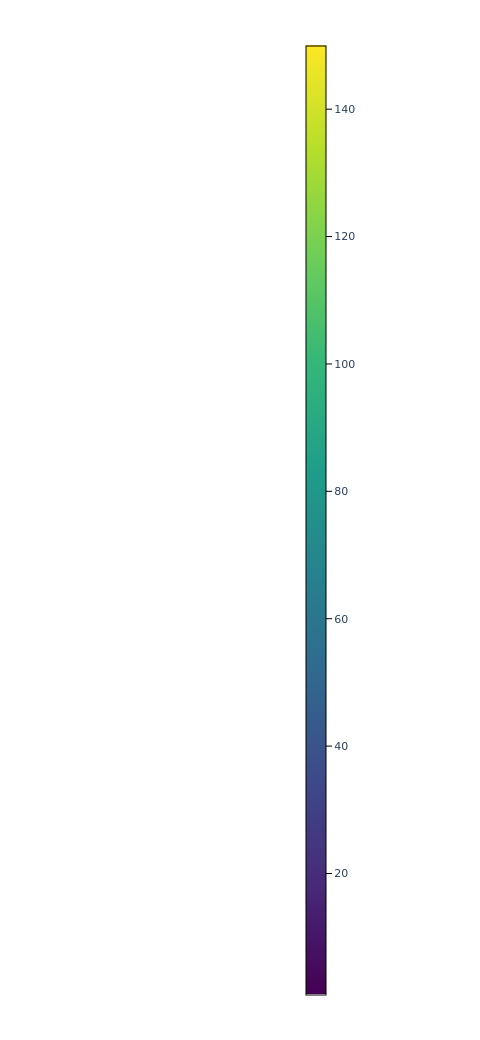
\includegraphics[width=0.7\linewidth]{legends/legend_pile-uncopyrighted__150.png}
\end{minipage}
\caption{Newline Position (150 chars) --- Gemma 2 9B, Layer 20. (A) E1749, Periodic Gain ($\Delta$per\,=\,0.320). (B) E1520, Periodic Gain ($\Delta$per\,=\,0.284).}
\end{figure*}
